\documentclass{article}

\usepackage{geometry}
\geometry{left=3cm,right=3cm,top=2cm,bottom=2cm}
\usepackage[utf8]{inputenc}
\usepackage{amsmath, amsfonts, amssymb, amsthm}
\usepackage[framemethod=default]{mdframed}% was framemethod=TikZ
\usepackage{mathrsfs}
\usepackage{comment}
\usepackage{enumerate}
\usepackage{xcolor}
\usepackage{titlesec}
\usepackage{setspace}
\usepackage{hyperref}
\hypersetup{
colorlinks=true,
allcolors=orange
}
\usepackage{cleveref}

\usepackage[most]{tcolorbox}
\usepackage{ragged2e}
\usepackage{todonotes}
\usepackage{cleveref}
\usepackage{mathtools}
\usepackage{svg, float}

\usepackage[sectionbib]{natbib}
\usepackage{chapterbib}


\definecolor{astral}        {RGB}{46,116,181}
\definecolor{cb-blue}       {RGB}{70, 130, 180}
\definecolor{orange}        {RGB}{214,150, 92}


% Name of the author!!!
\newcommand{\aut}{AUTHOR}

%
\titleformat*{\section}{\LARGE \bfseries}
\titleformat*{\subsection}{\Large \bfseries}
\titleformat*{\subsubsection}{\Large \bfseries}
% \titleformat*{\paragraph}{\large \bfseries}
\titleformat*{\subparagraph}{\large \bfseries}


%%%%%%%%%%%%%%%%%%%%%%%%%%%%%%%%%%%%%%%%%%%%%%%%%%%%%%%%%%%%
% General 
\newcommand{\nextline}{\hfill\break}
\newcommand{\nl}{\nextline\rm}
% \newcommand{\placeholder}{{\bf\color{red} NOOOOOOT COMPLEEEEEEET! COOOOOOOM BAAAAAACK!!!}}
\newcommand{\placeholder}{\todo{NOOOOOOT COMPLEEEEEEET! COOOOOOOM BAAAAAACK!!!}}
\newcommand{\inc}{{\color{red}Incomplete!!!}}

\DeclareMathOperator*{\esssup}{ess\,sup}

\newcommand{\defeq}{\stackrel{\text{def.}}{=}}
% FA and LA
% inner product: \inne{a}{b}
\newcommand{\inne}[2]{\left<{#1},{#2}\right>}

% norm: \norm{a}
\newcommand{\norm}[1]{\left\|{#1}\right\|}

% Curly H
\newcommand{\hbs}{$\mathscr{H}$ }
\newcommand{\hbp}{\mathscr{H}}

% Dual : \dual{x}
\newcommand{\dual}[1]{{#1}^*}

% Sequence from 1  to infty: \sequ{x_n}
\newcommand{\sequ}[1]{\left({#1}\right)_1^\infty}

% f: A-> B \func{f}{A}{B}
\newcommand{\func}[3]{${#1}:{#2}\xrightarrow{}{#3}$}

% interior
\newcommand{\interior}{\textrm{int}}

% Bounded linear funcs
\newcommand{\blf}[2]{\mathcal{L}({#1},{#2})}

\newcommand{\prf}{\textit{proof}:   }



% Fields 
\newcommand{\real}{\mathbb{R}}
\newcommand{\qq}{\mathbb{Q}}
\newcommand{\comp}{\mathbb{C}}
\newcommand{\inte}{\mathbb{Z}}
\newcommand{\natu}{\mathbb{N}}
%%%%%%%%%%%%%%%%%%%%%%%%%%%%%%%%%%%%%%%%%%%%%%%%%%%%%%%%%%%%



% If theoremstyle is n
    % Theorems
    % \newtheorem{example}{Example}[subsection]
    % \newtheorem{definition}[example]{Definition}
    % \newtheorem{proposition}[example]{Proposition}
    % \newtheorem{remark}[example]{Remark}
    % \newtheorem{theorem}[example]{Theorem}
    % \newtheorem{lemma}[example]{Lemma}
    % \newtheorem{corollary}[example]{Corollary}


% for numbering the theorems            
% \theoremstyle{plain}
% %%%%%%%%%%%%%%%%%%%%%%%%%%%%%%%%%%%%%%%%%%%%%%%%%%%%%%%%%%%
% \newtheorem{theorem}{Theorem}[section]
% \newtheorem{lemma}[theorem]{Lemma}
% \newtheorem{corollary}[theorem]{Corollary}
% \newtheorem{proposition}[theorem]{Proposition}
% %%%%%%%%%%%%%%%%%%%%%%%%%%%%%%%%%%%%%%%%%%%%%%%%%%%%%%%%%%%
% % the following are not in italics
% \theoremstyle{definition}
% \newtheorem{definition}[theorem]{Definition}
% \newtheorem{example}[theorem]{Example}
% \newtheorem{remark}[theorem]{Remark}
% \newtheorem{claim}[theorem]{Claim}
%%%%%%%%%%%%%%%%%%%%%%%%%%%%%%%%%%%%%%%%%%%%%%%%%%%%%%%%%%%%

% proof box
\newtcbtheorem[no counter]{pf}{Proof}{
  enhanced,
  rounded corners,
  attach boxed title to top,
  colback=white,
  colframe=black!25,
  fonttitle=\bfseries,
  coltitle=black,
  boxed title style={
    rounded corners,
    size=small,
    colback=black!25,
    colframe=black!25,
  } 
}{prf}
%%%%%%%%%%%%%%%%%%%%%%%%%%%%%%%%%%%%%%%%%%%%%%%%%%%%%%%%%%%%
% extra content box to put in contents not covered in the lecture notes
% use the command \begin{unexaminable}
\newmdenv[skipabove=7pt, skipbelow=7pt,
    rightline=false, leftline=false, topline=false, bottomline=false,
    backgroundcolor = gray!10,
    innerleftmargin=1in, innerrightmargin=1in, innertopmargin=5pt,
    leftmargin=-1in, rightmargin=-1in, linewidth=4pt,
    innerbottommargin=5pt]{unexamBox}
\newenvironment{unexaminable}{\begin{unexamBox}}{\end{unexamBox}}

%%%%%%%%%%%%%%%%%%%%%%%%%%%%%%%%%%%%%%%%%%%%%%%%%%%%%%%%%%%%
% clever ref settings
\crefname{lemma}{lemma}{lemmas}
\Crefname{lemma}{Lemma}{Lemmas}
\crefname{theorem}{theorem}{theorems}
\Crefname{theorem}{Theorem}{Theorems}
%%%%%%%%%%%%%%%%%%%%%%%%%%%%%%%%%%%%%%%%%%%%%%%%%%%%%%%%%%%%
% formatting 
% https://tex.stackexchange.com/questions/217497/aligning-stackrel-signs-beneath-each-other-using-split
\newlength{\leftstackrelawd}
\newlength{\leftstackrelbwd}
\def\leftstackrel#1#2{\settowidth{\leftstackrelawd}%
{${{}^{#1}}$}\settowidth{\leftstackrelbwd}{$#2$}%
\addtolength{\leftstackrelawd}{-\leftstackrelbwd}%
\leavevmode\ifthenelse{\lengthtest{\leftstackrelawd>0pt}}%
{\kern-.5\leftstackrelawd}{}\mathrel{\mathop{#2}\limits^{#1}}}
%%%%%%%%%%%%%%%%%%%%%%%%%%%%%%%%%%%%%%%%%%%%%%%%%%%%%%%%%%%%

%%%%%%%%%%%%%%%%%%%%%%%%%%%%%%%%%%%%%%%%%%%%%%%%%%%%%%%%%%%%
% colors
\usepackage{xcolor}
\definecolor{royal}{RGB}{0,35,102}
\definecolor{navyblue}{cmyk}{1,0.5,0,0.3}
\definecolor{c0}{cmyk}{0.83, 0.34, 0, 0.29}
\definecolor{c1}{cmyk}{0, 0.5, 0.95, 0}
\definecolor{c2}{cmyk}{0.72, 0, 0.72, 0.37}
\definecolor{skyblue}{cmyk}{0.6,0.16,0,0}
\definecolor{lightgreen}{cmyk}{0.5,0,0.5,0}
\definecolor{pastelgreen}{cmyk}{0.25,0,0.25,0}
\definecolor{mossgreen}{cmyk}{0.64,0.4,1,0}
\definecolor{reddish}{cmyk}{0, 0.64, 0.64, 0.2}
\definecolor{one}{cmyk}{0, 0.6, 0.46, 0.69}
\definecolor{two}{cmyk}{0.11, 0, 0.72, 0.16}
\definecolor{imperialorange}{RGB}{255,134,24}
%%%%%%%%%%%%%%%%%%%%%%%%%%%%%%%%%%%%%%%%%%%%%%%%%%%%%%%%%%%%
% spacing
\onehalfspacing
\RaggedRight
%%%%%%%%%%%%%%%%%%%%%%%%%%%%%%%%%%%%%%%%%%%%%%%%%%%%%%%%%%%%


% modify innerrightmargin if floats were lost

\usepackage{amsfonts, amsmath, amssymb, amsthm, thmtools, bm}
\usepackage{avant} % Use the Avantgarde font for headings
\usepackage[most]{tcolorbox}

% Boxed/framed environments
\newtheoremstyle{royalnumbox}%
{0pt}% Space above
{0pt}% Space below
{\normalfont}% Body font
{}% Indent amount
{\small\bf\color{royal}}% Theorem head font
{\;}% Punctuation after theorem head
{0.25em}% Space after theorem head
{ \color{royal} 
    \thmname{#1} 
    \thmnumber{#2} \thmnote{\bfseries\color{black}---\nobreakspace#3.}} % Optional theorem note
\renewcommand{\qedsymbol}{$\blacksquare$}% Optional qed square

\newtheoremstyle{blacknumex}% Theorem style name
{5pt}% Space above
{5pt}% Space below
{\normalfont}% Body font
{} % Indent amount
{\small\bf}% Theorem head font
{\;}% Punctuation after theorem head
{0.25em}% Space after theorem head
{
    \thmname{#1}
    \thmnumber{#2}
    \thmnote{---\nobreakspace#3.}}% Optional theorem note

\newtheorem*{notation}{Notation}
\newtheorem*{hint}{Hint}
\newtheorem*{solution}{Solution}

\newcounter{dummy} 
\numberwithin{dummy}{section}

\theoremstyle{royalnumbox}
\newtheorem{definitionT}[dummy]{Definition}
\newtheorem{theoremT}[dummy]{Theorem}
\newtheorem{lemmaT}[dummy]{Lemma}
\newtheorem{corollaryT}[dummy]{Corollary}
\newtheorem{propositionT}[dummy]{Proposition}
\newtheorem{propertyT}[dummy]{Property}
\newtheorem{remarkT}[dummy]{Remark}

\theoremstyle{blacknumex}
\newtheorem{exampleT}[dummy]{Example}
\newtheorem{exerciseT}[dummy]{Exercise}

\numberwithin{equation}{section}

\RequirePackage[framemethod=TikZ]{mdframed}

\newcounter{definition}

% % Definition box
% \newtcolorbox{dBox}{
%   enhanced,
%   breakable,
%   arc=5pt, outer arc=5pt,
%   colback=reddish!10, 
%   colframe=reddish,
%   boxrule=1pt,
%   left=5pt, 
%   right=5pt, 
%   top=5pt, 
%   bottom=5pt,
% %   skipabove=7pt, skipbelow=7pt
% }



% % Main Theorem box
% \newtcolorbox{tBox}{
%   enhanced,
%   breakable,
%   arc=5pt, 
%   outer arc=5pt,
%   colback=c0!10, 
%   colframe=c0!10,
%   boxrule=1pt,
%   left=5pt, 
%   right=5pt, 
%   top=5pt, 
%   bottom=5pt,
% %   skipabove=7pt, skipbelow=7pt
% }


% % Lemma/Corollary/Proposition/Property box
% \newtcolorbox{lBox}{
%   enhanced,
%   breakable,
%   arc=5pt,
%   outer arc=5pt,
%   colback=c0!10,
%   colframe=c0!10,
%   boxrule=1pt,
%   left=5pt,
%   right=5pt,
%   top=5pt,
%   bottom=5pt,
% %   skipabove=7pt, skipbelow=7pt
% }

% % Example/Remark/Exercise box
% \newtcolorbox{exBox}{
%   enhanced,
%   breakable,
%   arc=5pt, 
%   outer arc=5pt,
%   colback=mossgreen!10!white,
%   colframe=mossgreen,
%   boxrule=1pt,
%   left=5pt,
%   right=5pt,
%   top=5pt,
%   bottom=5pt,
% %   skipabove=7pt, skipbelow=7pt
% }

% % Extra content box for contents not covered in the lecture notes
% \newtcolorbox{unexamBox}{
%   enhanced,
%   breakable,
%   arc=20pt, 
%   outer arc=20pt,
%   colback=gray!10,
%   colframe=gray,
%   boxrule=1pt,
%   left=5pt, 
%   right=5pt, 
%   top=5pt, 
%   bottom=5pt,
% %   skipabove=7pt, skipbelow=7pt
% }

% Definition box
\newtcolorbox{dBox}{
  enhanced,
  breakable,
  arc=5pt, outer arc=5pt,
  colback=skyblue!10,  % Light blue
  colframe=skyblue,    % Blue
  boxrule=1pt,
  left=5pt, 
  right=5pt, 
  top=5pt, 
  bottom=5pt,
}

% Main Theorem box
\newtcolorbox{tBox}{
  enhanced,
  breakable,
  arc=5pt, 
  outer arc=5pt,
  colback=yellow!10,   % Light yellow
  colframe=yellow!80!black, % Dark yellow
  boxrule=1pt,
  left=5pt, 
  right=5pt, 
  top=5pt, 
  bottom=5pt,
}

% Lemma/Corollary/Proposition/Property box
\newtcolorbox{lBox}{
  enhanced,
  breakable,
  arc=5pt,
  outer arc=5pt,
  colback=orange!10,   % Light orange
  colframe=orange!80!black, % Dark orange
  boxrule=1pt,
  left=5pt,
  right=5pt,
  top=5pt,
  bottom=5pt,
}

% Example/Remark/Exercise box
\newtcolorbox{exBox}{
  enhanced,
  breakable,
  arc=5pt, 
  outer arc=5pt,
  colback=teal!10!white,   % Light teal
  colframe=teal,           % Teal
  boxrule=1pt,
  left=5pt,
  right=5pt,
  top=5pt,
  bottom=5pt,
}

% Extra content box for contents not covered in the lecture notes
\newtcolorbox{unexamBox}{
  enhanced,
  breakable,
  arc=20pt, 
  outer arc=20pt,
  colback=gray!10,    % Light gray
  colframe=gray,      % Gray
  boxrule=1pt,
  left=5pt, 
  right=5pt, 
  top=5pt, 
  bottom=5pt,
}

\newenvironment{unexaminable}{\begin{unexamBox}}{\end{unexamBox}}




% Creates an environment for each type of theorem and assigns it a theorem text style from the "Theorem Styles" section above and a colored box from above
\newenvironment{definition}{\begin{dBox}\begin{definitionT}}{\end{definitionT}\end{dBox}}

\newenvironment{theorem}{\begin{tBox}\begin{theoremT}}{\end{theoremT}\end{tBox}}

\newenvironment{lemma}{\begin{lBox}\begin{lemmaT}}{\end{lemmaT}\end{lBox}}

\newenvironment{proposition}{\begin{lBox}\begin{propositionT}}{\end{propositionT}\end{lBox}}

\newenvironment{corollary}{\begin{lBox}\begin{corollaryT}}{\end{corollaryT}\end{lBox}}

\newenvironment{property}{\begin{lBox}\begin{propertyT}}{\end{propertyT}\end{lBox}}


\newenvironment{remark}{\begin{exBox}\begin{remarkT}}{\end{remarkT}\end{exBox}}

\newenvironment{example}{\begin{exBox}\begin{exampleT}}{{}\end{exampleT}\end{exBox}}
\usepackage{tikz}
\usepackage{algorithm}
\usepackage{algpseudocode}

\title{Week 5}

\date{\today}


\begin{document}

\maketitle

\section{Threshold Behaviours} 

We begin with an example of a threshold behaviour in a random graph.  

\begin{example}
    In $G(n,p)$, if $p=\frac{c}{n}$ with $c<1$, then the largest connected component is of size $O(\log n)$, whereas if $c>1$, then the largest connected component is of linear size with probability $1$ as $n\to \infty$.      
\end{example}

To show this, we use the approach in \citep{krivelevich2012phase} and use the Depth-First Search (DFS) algorithm on the random graph. 

\subsection{Depth-First Search}
The DFS operates on the vertex set $V$ with three sets of vertices at each step:
\begin{itemize}
    \item $S$ is the set that has been explored
    \item $T$ is the set of vertices to be explored
    \item $U = V\setminus (S\cup T)$ is the set of vertices under investigation
\end{itemize}

The algorithm starts with $S=\emptyset$, $T=V$ and $U=\emptyset$. At each step, if $U$ is nonempty, let $v$ be the last vertex added to $U$, we perform the following:
\begin{enumerate}
    \item If $v$ has a neighbour $u$ in $T$, move $u$ from $T$ to $U$.
    \item If $v$ has no neighbour in $T$, move $v$ from $U$ to $S$.
\end{enumerate}

If $U$ is empty, we pick a vertex $v$ from $T$ and move it to $U$ (select the vertex with the smallest index). If $U\cup T=\emptyset$, query all remaining pairs in $S$ and stop.  

The period of time between two consecutive emptyings of $U$ is called an \textbf{epoch}, which reveals a connected component.  

\begin{proposition}
    The DFS algorithm has the following properties:
    \begin{enumerate}
        \item The number of epochs is equal to the number of connected components.
        \item There are no edges between sets $S$ and $T$ at any time.
        \item The set $U$ always spans a path.
    \end{enumerate}
\end{proposition}

\begin{proof}
    Those directly follow from the algorithm.
\end{proof}

This particular formulation of the DFS algorithm allows for the application on an Erd\H{o}s-R\'{e}nyi random graph, where we query the existence of an edge between two vertices by a Bernoulli trial with probability $p$.  

Denote $X_i\in \{0,1\}$ as the outcome of the $i$-th query, with each $X_i \sim \text{Bernoulli}(p)$ for $i=1, \ldots, \binom{n}{2}$. 

\begin{proposition}
    Let $S(t), U(t), T(t)$ be the sets at time $t$ in the DFS algorithm. Then, 
    \begin{equation*}
        |U(t)|\leq1+\sum_{i=1}^{t}X_{i} \quad \mathrm{and} \quad |S(t)\cup U(t)|\geq\sum_{i=1}^{t}X_{i}
    \end{equation*}
    At all times, $|S(t)|+|U(t)|+|T(t)|=n$.
\end{proposition}

The $1$ comes from the initial vertex $v$ in $U$ at the beginning of each epoch. 

\subsection{Small Connected Components}

We will first show that the size of any connected component cannot exceed some constant associated with the probability $p$ with high probability as $n\to \infty$.  

\begin{theorem}\label{thm:small_connected_components}
    Let $\varepsilon \in (0,1)$ be fixed and let $G\sim G(n,p)$ with $p=\frac{1-\varepsilon}{n}$, then any connected component $C$ of $G$, satisfies
    \begin{equation*}
        \mathbb{P}(|C|\leq \frac{7}{\varepsilon^2}\log n)\to 1 \quad \text{as} \quad n\to \infty
    \end{equation*}
\end{theorem}

The proof of this theorem is based on the following lemma, which bounds the number of successes $W$ in an interval of length $\ell$ during a sequence of Bernoulli trials.  

\begin{lemma}\label{lem:bernoulli_trials}
    Let $X_1, \ldots, X_N \overset{i.i.d.}{\sim} \text{Bernoulli}(p)$. Let $k, \ell \in \mathbb{N}$ with $k > \ell p$. Then, define the random variable $Y_t$ as:
    \begin{equation*}
        Y_t = \sum_{i=t}^{t+\ell-1}X_i
    \end{equation*}
    for $t=1, \ldots, N-\ell+1$. And the random variable $W$ as:
    \begin{equation*}
        W = \sum_{t=1}^{N-\ell+1} \mathbf{1}_{\{Y_t\geq k\}}
    \end{equation*}
    Then,
    \begin{equation*}
        \mathbb{P}(W\geq 1)\leq (N-\ell+1)\exp\left(-\frac{(k-\ell p)^2}{2(\ell p + (k - \ell p ) / 3)}\right)
    \end{equation*}
\end{lemma}

We delay the proof of this lemma to the end of this section and first prove \Cref{thm:small_connected_components}.  

\begin{proof}[Proof of \Cref{thm:small_connected_components}]
    Assume for the sake of contradiction that $G$ contains a connected component $C$ with more than $\frac{7}{\varepsilon^2}\log n$ vertices.  Let $k+1=\lfloor \frac{7}{\varepsilon^2}\log n \rfloor + 1$ be the smallest integer which is larger than $\frac{7}{\varepsilon^2}\log n$. We show the probability of such a component to exist tends to $0$ as $n\to \infty$.  

    \medskip

    During the epoch when $C$ was created, consider the moment when the algorithm has received a positive response for the $(k+1)$-th time (the $k+1$-th vertex of $C$ is found). 
    % Let $\Delta S = S\cap C$ be the set of vertices in $C$ that have been found before this moment, then $|\Delta S \cup U| = k$, 
    Before this moment the algorithm has recevied exactly $k$ positive responses.  

    The total number of queries up to this moment during this epoch is at most

    \begin{equation*}
        \binom{k}{2} + k(n-k) < kn
    \end{equation*}

    Set $\ell = kn$ and $N=\binom{n}{2}$, then by \Cref{lem:bernoulli_trials}, we have such a component $C$ with probability at most

    \begin{align*}
        \binom{n}{2} \exp \left( -\frac{(k-\ell p)^2}{2(\ell p + (k-\ell p)/3)} \right) &= \binom{n}{2} \exp\left(-\frac{k\varepsilon^2}{2(1-2\varepsilon/3)}\right) \\
        &\leq \binom{n}{2} \exp\left(\frac{k\varepsilon^2}{2(1-2\varepsilon/3)} - \frac{7 \log n}{2 (1-2\varepsilon/3)}\right) \\
    \end{align*}

    as $k\geq \frac{7}{\varepsilon^2}\log n - 1$. Now note $\binom{n}{2} < n^2$ and $\varepsilon<1$, so the probability of such a component $C$ existing is at most
    \begin{equation*}
        n^2 \exp\left(\frac{k\varepsilon^2}{2(1-2\varepsilon/3)}\right) n^{-7/2(1-2\varepsilon/3)} < e^{3/2} n^{-3/2}
    \end{equation*}

    Letting $X$ denote the number of connected components of size at least $\frac{7}{\varepsilon^2}\log n$, we have by Markov's inequality that
    \begin{equation*}
        \mathbb{P}(X\geq 1) \leq \mathbb{E}(X) < e^{3/2} n^{-1/2}
    \end{equation*}

    which tends to $0$ as $n\to \infty$.
\end{proof}

To show \Cref{lem:bernoulli_trials}, we require the following Chernoff bound.  

\begin{lemma}\label{lem:chernoff}
    If $X\sim \text{Binomial}(N,p)$, then for any $N, k >0$,
    \begin{equation*}
        \mathbb{P}(X-N p\geq k)\leq \exp\left(-{\frac{k^{2}}{2(N p+k/3)}}\right)
    \end{equation*}
\end{lemma}

The proof of this lemma is given in problem sheet 0.  

\begin{proof}[Proof of \Cref{lem:bernoulli_trials}]
    Let $W$ denote the number of intervals of length $\ell \in \{1, \ldots, N\}$ in which at least $k$ of the random variables $X_i$ take the value 1. We want to bound $\mathbb{P}(W \geq 1)$ from above.

    Using Markov's inequality,
    \[
    \mathbb{P}(W \geq 1) \leq \mathbb{E}(W).
    \]
    
    Now
    \[
    \mathbb{E}(W) = (N - \ell + 1)\mathbb{P}\left(\sum_{i=1}^{\ell} X_i \geq k \right).
    \]
    
    From \Cref{lem:chernoff}, we have
    \[
    \mathbb{P}\left(\sum_{i=1}^{\ell} X_i \geq k\right) = \mathbb{P}\left(\sum_{i=1}^{\ell} X_i - \ell p \geq k - \ell p\right) \leq \exp \left(-\frac{(k-\ell p)^2}{2(\ell p+(\ell p)^2/3)}\right)
    \]
    
    Combining these bounds yields the assertion.
\end{proof}


\begin{remark}
    The proof of \Cref{thm:small_connected_components} is based on the fact that the DFS algorithm must receive $k$ positive responses during \textbf{an interval/window within the epoch for that connected component} among the queries to ensure a size of at least $k$.
\end{remark}


\subsection{Large Connected Components}

We also state another result from \citep{krivelevich2012phase} that shows the existence of a linear size connected component with high probability as $n\to \infty$.  

\begin{theorem}
    Let $\varepsilon \in (0,\frac{1}{10})$ be fixed and let $G\sim G(n,p)$ with $p=\frac{1+\varepsilon}{n}$, let the largest connected component be $C_{\max}$. Then,
    \begin{equation*}
        \mathbb{P}(|C_{\max}|\geq \frac{1}{5}\varepsilon^2 n)\to 1 \quad \text{as} \quad n\to \infty
    \end{equation*}
\end{theorem}

The proof can be found in the lecture notes which is not examinable.

\section{Shortest Paths}
In this section, we study the distribution of the length of the shortest path between two vertices in a Newman-Watts-Strogatz (NWS) random graph. The important idea is to use continuous-time analysis for discrete-time processes.  

\subsection{First Simplification}

We consider the continuous circle model from \citep{Newman_2000}: let $C$ be a circle of circumference $L$. A $\mathrm{Poisson}(L\rho/2), L\rho>1$ number of shortcuts are added uniformly at random to the circle. The chords between points have length zero. 

\begin{figure}[h]
    \centering
    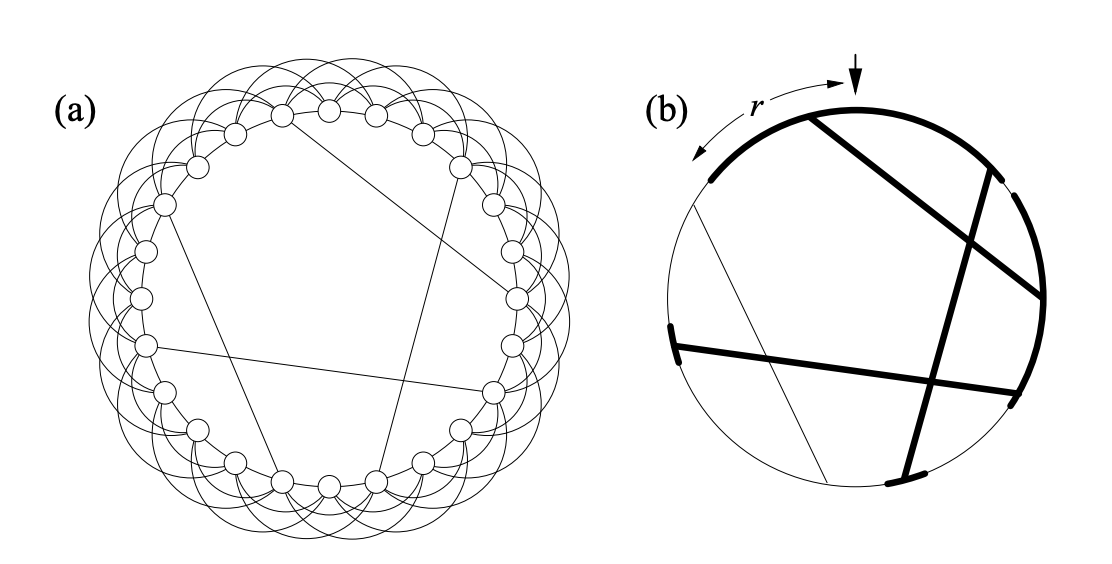
\includegraphics[width=0.7\textwidth]{figures/newman1999.png}
    \caption{The continuous circle model \citep{Newman_2000}}
    \label{fig:newman1999}
\end{figure}

For two randomly chosen points $P$ and $Q$ on the circle, we are interested in the distribution of the length of the shortest path $\mathcal{D}$ between them.  

\subsection{Second Simplification}


\subsection{Poisson Approximation}


\subsection{Unconditioning}





\newpage
\bibliographystyle{apalike}
\bibliography{bibliography4.bib}
\end{document}